\subsection{Comparación entre aprendizaje automático tradicional y aprendizaje profundo}

Una vez expuestos los modelos tradicionales de clasificación, sus limitaciones en escenarios reales y el panorama general del aprendizaje profundo en tareas de visión por computadora, resulta adecuado establecer una comparación directa entre ambos enfoques. Esta comparación tiene como propósito precisar, de forma puntual, las diferencias en la manera en que el aprendizaje automático tradicional y el aprendizaje profundo representan la información, aprenden características y responden ante problemas visuales complejos. De esta manera, se busca reforzar con mayor claridad la justificación del aprendizaje profundo como el enfoque más adecuado para el problema planteado en el presente proyecto.

\subsubsection{Similitudes generales entre ambos enfoques}

Tanto el aprendizaje automático tradicional como el aprendizaje profundo se apoyan en conjuntos de datos para entrenar algoritmos capaces de encontrar relaciones entre entradas y salidas. En ambos casos, el modelo aprende a partir de ejemplos de entrenamiento con el fin de generalizar ese conocimiento hacia nuevos datos no vistos. Asimismo, ambos enfoques forman parte de la inteligencia artificial y la ciencia de datos, y pueden emplearse para resolver tareas que resultarían costosas o poco prácticas mediante métodos tradicionales de programación \cite{aws2026ml_vs_dl}.

\begin{figure}[H]
    \centering
    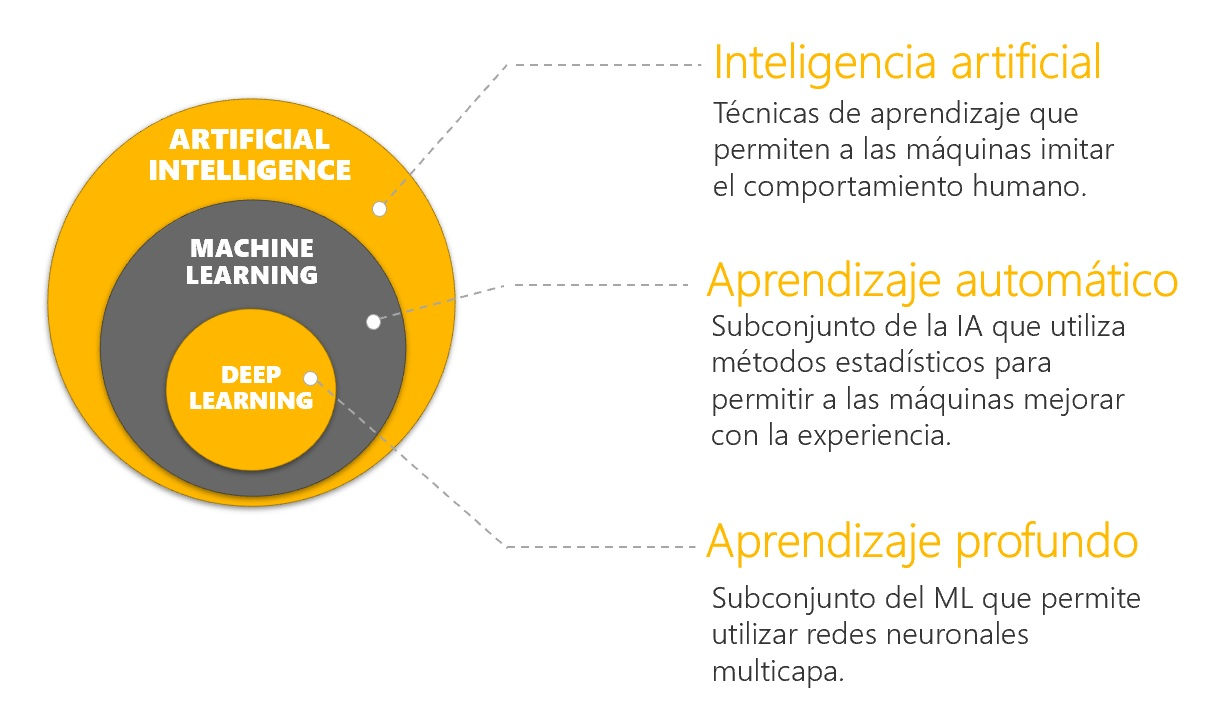
\includegraphics[width=0.7\textwidth]{images/C4/conjuntosIA.png}
    \caption{Subconjuntos de la Inteligencia artificial. Tomado de \cite{bravent2019redes_neuronales}}
    
\end{figure}


De igual manera, tanto el \textbf{machine learning} como el \textbf{aprendizaje profundo} se apoyan en fundamentos matemáticos y estadísticos para construir sus modelos. Esto incluye el uso de técnicas relacionadas con el análisis de regresión, el álgebra lineal, el cálculo y otros métodos numéricos que permiten optimizar el proceso de aprendizaje. En ambos casos, la calidad y cantidad de los datos disponibles influye directamente en el desempeño final del sistema \cite{aws2026ml_vs_dl}.


\subsubsection{Diferencias en el enfoque de resolución de problemas}

A pesar de compartir una base común, la principal diferencia entre ambos enfoques radica en la forma en que abordan la representación de la información. En el aprendizaje automático tradicional, es habitual que exista una etapa de ingeniería de características, en la cual una persona selecciona, diseña o extrae manualmente los atributos que serán utilizados por el modelo. Esto implica que parte del conocimiento necesario para resolver el problema debe ser definido explícitamente antes del entrenamiento \cite{aws2026ml_vs_dl}.

En cambio, el aprendizaje profundo reduce esta dependencia al permitir que el propio modelo aprenda automáticamente las representaciones más relevantes a partir de los datos. Esto se logra mediante arquitecturas basadas en redes neuronales profundas, las cuales están compuestas por múltiples capas capaces de transformar progresivamente la información de entrada en representaciones de mayor nivel de abstracción. De esta manera, la extracción de características y la clasificación dejan de ser procesos separados y pasan a integrarse dentro de un mismo esquema de aprendizaje \cite{aws2026ml_vs_dl}.

Bajo esta premisa, puede decirse que el aprendizaje profundo representa una evolución del aprendizaje automático hacia modelos con mayor capacidad de representación. Mientras que los algoritmos tradicionales suelen depender de variables explícitas o de características previamente construidas, los modelos profundos pueden aprender por sí mismos patrones más complejos y menos evidentes dentro de los datos \cite{aws2026ml_vs_dl}.

\subsubsection{Diferencias en los datos, entrenamiento e infraestructura}

Otra diferencia importante entre ambos enfoques tiene que ver con el tipo de datos para el cual suelen resultar más adecuados. El aprendizaje automático tradicional suele ofrecer buenos resultados en problemas bien definidos que trabajan con \textbf{datos estructurados}, como tablas o registros con variables numéricas y categóricas claramente establecidas. Por otro lado, el aprendizaje profundo resulta más apropiado cuando se trabaja con \textbf{datos no estructurados}, tales como imágenes, audio o texto, donde se requiere un nivel mayor de abstracción para identificar patrones relevantes \cite{aws2026ml_vs_dl}.

En lo que respecta al entrenamiento, los modelos de aprendizaje profundo suelen demandar más datos, más tiempo de cómputo y una infraestructura más compleja que los modelos tradicionales. Esto se debe a que las redes neuronales profundas involucran una mayor cantidad de operaciones matemáticas y parámetros ajustables, lo que incrementa el costo computacional del entrenamiento. Por el contrario, muchos \textbf{algoritmos clásicos de machine learning} pueden entrenarse con menor volumen de datos y con menores requerimientos computacionales \cite{aws2026ml_vs_dl}.

Sin embargo, esta mayor complejidad también se traduce en una mayor capacidad para modelar relaciones no lineales y patrones de alta complejidad. Por ello, aunque el aprendizaje profundo exige más recursos, su uso se justifica cuando la naturaleza del problema supera la capacidad representacional de los enfoques tradicionales \cite{aws2026ml_vs_dl}.